%%%%%%%%%%%%%%%%%%%%%%%%%%%%%%%%%%%%%%%%%%%%%%%%%%%%%%%%%%%%%%%%%%%%%%%%%%%%%%%%%%%%%%%%
%                        ELECTRIMACS 2024 TEMPLATE FILE                                %
%                              Version 1.01 - 2023.10.24                                  %
%%%%%%%%%%%%%%%%%%%%%%%%%%%%%%%%%%%%%%%%%%%%%%%%%%%%%%%%%%%%%%%%%%%%%%%%%%%%%%%%%%%%%%%%

%
% This is a template file for the conference ELECTRIMACS 2024 Castellon conference.
% The template is developed starting from LaTeX package SVJour3 for Springer journals.
%
% Copy it to a new file with a new name and use it as the basis for your article.
% Delete % signs as needed.
%


% ======================================================================================
% Please DO NOT MODIFY the options in this section
\RequirePackage{fix-cm}
\documentclass[smallextended,twocolumn]{electrimacs2024}
\smartqed  % flush right qed marks, e.g. at end of proof
\usepackage{mathptmx}      % use Times fonts if available on your TeX system
% ======================================================================================


% --------------------------------------------------------------------------------------
% Insert here the call for the packages your document requires
\usepackage{amsmath}
\usepackage{graphicx}
%\usepackage{latexsym}
%\usepackage{amsthm,amsfonts,graphicx,colordvi,color,multirow,amssymb}
% etc.
%
% --------------------------------------------------------------------------------------

% --------------------------------------------------------------------------------------
% Place your own definitions here and don't use \def but \newcommand{}{}
\newcommand{\figref}[1]{Fig. \ref{#1}}
\newcommand{\tabref}[1]{Tab. \ref{#1}}
%
% --------------------------------------------------------------------------------------



\begin{document}

% --------------------------------------------------------------------------------------
% Set the following information:
% 1. Title
% 2. Authors
% 3. Affiliations
%
\title{Day Ahead Energy Trading in Community Microgrids Using Smart Contracts}

\author{Bashar AL MOHAMMAD \and Berk CELIK}

\institute{F.  Author \and T. Author \at
  DESID -- Universitat Jaume I\\
 Av. Vicent Sos Baynat, s/n 12071 Castell\'on de la Plana, Spain \\
              \email{fauthor@somewhere.org, tauthor@elsewhere.com}
              \and
           S. Author \and L. Author \at
              Institution name\\
              address line 1\\
              address line 2, if needed\\
              Zip code, City, Province, Country\\
              \email{\ldots}
}
\maketitle
% --------------------------------------------------------------------------------------


\begin{abstract}
The abstract should summarize the content of the paper, indicating its
aim, starting point, original contribution and conclusions (up to 200 words).
\end{abstract}

\section{Introduction}
This document briefly describes how to write a manuscript for ELECTRIMACS 2024 Castell\'on conference.


\section{How to prepare your manuscript}


\subsection{Templates}
Authors are kindly invited to use the \LaTeX source file (TEX) or Word templates (DOCX) available on the conference website:
\begin{center}
\texttt{https://electrimacs2024.uji.es/}.
\end{center}
The use of LaTeX \emph{is highly recommended} for manuscript preparation.

This is the template version 1.0 – May 2023.

\subsection{Manuscript information}
Authors are kindly asked to prepare their manuscript according to the following specifications:
\begin{itemize}
  \item Language: English
  \item Size: A4
  \item Two columns
  \item Length: from four (4) to six (6) pages.
\end{itemize}

\subsection{Document size and style}
The document margin and column size are summarised in \tabref{TAB:colsandmargins}. Font, style and size of titles and texts are reported in \tabref{TAB:sizeandstyle}.
\begin{table}[!hb]
	\centering
	\caption{Colums and margins}\label{TAB:colsandmargins}
	\begin{tabular}{p{1.5in} p{1.1in}}
\hline\hline
    \textbf{Parameter}  & \textbf{Value}\\ \hline\hline
    Left margin   & 15 mm\\
	Right margin  & 21 mm\\
	Upper margin  & 30 mm\\
	Lower margin  & 31 mm\\ \hline
	First page upper margin  & 47 mm\\
    Blank space after authors' line & 43 mm\\
    Column width  & 84 mm\\
    Column separation & 6 mm\\
    Figure width  & $\le$84 mm\\ \hline\hline
	\end{tabular}
\end{table}

\begin{table}[!ht]
	\centering
	\caption{Document style} \label{TAB:sizeandstyle}
	\begin{tabular}{p{1.3in} p{1.3in}} 	\hline\hline
	\textbf{Style}                      & \textbf{Characteristics}         \\ \hline\hline
	Paper Title                         & 16 pt, bold, left-aligned\\ \hline
	Authors' names                      & 10 pt, bold, left-aligned           \\ \hline
	Affiliation and e-mail              & 8.5pt, left-aligned in the footnote in column one\\ \hline
	Section title                       & 10 pt, bold, left-aligned, hierarchically numbered  \\ \hline
	Subsection title                    & 10 pt, italic, left-aligned, hierarchically numbered  \\ \hline
	Main body text                      & 10 pt, justified, single-spaced \\ \hline
	Acknowledgements section title      & 8.5 pt, bold \\ \hline
	Acknowledgements body text          & 8.5 pt, justified \\ \hline
	Figure and table title              & 8.5 pt, bold       \\ \hline
	Figure and table captions           & 8.5 pt, justified \\ \hline\hline
	\end{tabular}
\end{table}

\subsection{Submission of papers}
A camera-ready PDF manuscript must be submitted for review through the conference submission system. No other file format is accepted for this initial submission. You will find more information about initial submission on the conference website \emph{Papers $>$ Submission}.

\subsection{Figure, tables, citations and cross reference}

\begin{figure}[!ht]
\centering
  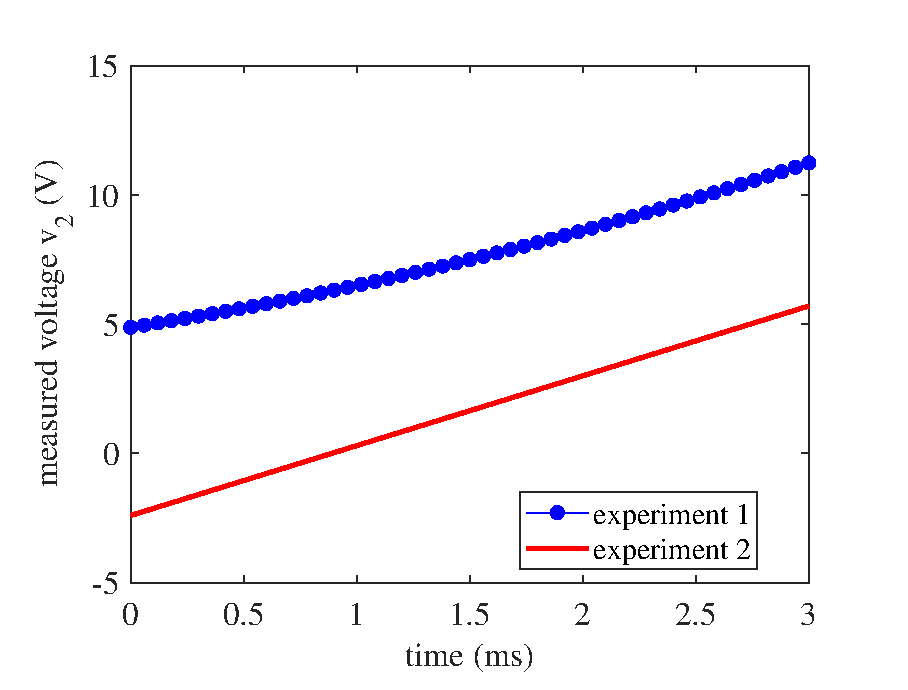
\includegraphics[width=8.4cm]{figures/graph1.eps}\\ % please do not exceed 8.4cm width. Do not use \columnwidth.
  \caption{Please write the caption here. If the caption is long, the text of the caption is justified.}\label{FIG:graph1}
\end{figure}%

\begin{figure}[!ht]
\centering
  \includegraphics[width=7.0cm]{figures/photo2.jpg}\\ % please do not exceed 8.4cm width. Do not use \columnwidth.
  \caption{Experimental setup.}\label{FIG:photo2}
\end{figure}%

Refer to a figure using \figref{FIG:graph1}, or \figref{FIG:photo2}. Refer to a table using \tabref{TAB:colsandmargins}.
You can cite an item listed in the Reference section as \cite{Teulings1997} or \cite{Maniktala2006,Cousseau2017}.

\subsection{Equations}
Equations are left-aligned and numbered as shown below:
\begin{align}
\left(\frac{R_e}{1-D}+\frac{DT_s}{C_e}\right)\le \Delta v_{pp}^{max}.\label{EQ:waveformDVpp}
\end{align}
Please refer to an equation using \eqref{EQ:waveformDVpp}.

\section{Section title}
ELECTRIMACS 2024 is an international conference on theory and application of modelling, simulation, analysis, design optimization, identification and diagnostics in electrical power engineering.

\subsection{Subsection title}
Application of interest include, but are not limited to:
\begin{itemize}
\item  electric machines and electromagnetic devices
\item  power electronics
\item  transportation systems
\item  smart grids
\item  electric and hybrid vehicles
\item  renewable energy systems
\item  energy storage, batteries, supercapacitors and fuel cells
\item  wireless power transfer
\end{itemize}


\section{ELECTRIMACS 2024 Topics}

\subsection{Modelling, Simulation and Identification}
\begin{itemize}
\item Diagnostics in electrical systems 
\item Modelling methods and software development
\item Modelling and simulation of power systems, power electronics and drives, distributed generating systems, electric machines and transformers, batteries and fuel cell systems
\item Electromagnetic fields and compatibility
\item Emerging electrical technologies
\item Simulation methodologies for design and analysis of electromagnetic devices
\item Hardware in the loop emulation
\item Thermal problems
\end{itemize}
 

 \subsection{Systems’ Design and Optimization}
\begin{itemize}
\item System identification and optimization methods and theory
\item Computer-aided design and optimization of power converters, protections, energy storage systems, electric machines, power systems
\item Multiphysics issues
\item Power system and power converter architectures
\item Methods and techniques for energy management  
\end{itemize}

 \subsection{Control and Power Management}
\begin{itemize}
\item Optimal, feedback, and stochastic control
\item Filtering
\item Linear and nonlinear systems control and programming
\item Digital implementation and control applied to electrical systems
\item Real time simulation methods
\item Rapid control prototyping of electrical systems
\item Embedded systems
\item Fuzzy logic and applications
\item Genetic algorithms and evolutionary computing
\item Model predictive, robust, sliding mode networked control of electrical systems and machines
\item Identification/diagnostic/prognostic techniques applied to electrical systems
\item Power quality
\end{itemize}


\subsection{Numerical Methods and Machine Learning}
\begin{itemize}
\item Artificial intelligence’s potential to boost electrical systems performance
\item Grid condition monitoring and predictive maintenance
\item Electrical market variables pattern recognition
\item Energy storage systems degradation analysis
\item Renewable energy generation and electric demand forecast
\item Applications in electric vehicles
\item Estimation of state-of-charge and state-of-health in batteries; signal modelling
\item Robot locomotion
\item Electrical systems’ parameter identification
\item Energy flows prediction
\item Electrical faults forecasting
\end{itemize}


\section{Conclusions}
Write your conclusions here.

\begin{acknowledgements}
You can write your acknowledgements here, if necessary.
\end{acknowledgements}




% Non-BibTeX users please use
\begin{thebibliography}{}
%
% and use \bibitem to create references.
%
\bibitem{Teulings1997} % this is a paper
W. Teulings, J.L. Schanen, J. Roudet, %
``Analysis of the Current Distribution Between Paralleled Capacitors in a Chopper on Printed Circuit Board'',%
\emph{IEEE Industry Applications Society Annual Meeting New Orleans},%
pp. 1066-72, 1997.
%
\bibitem{Maniktala2006}
S. Maniktala, %
\emph{Switching Power Supplies A to Z -- Second Edition},%
Waltham, 2012.
%
\bibitem{Cousseau2017}
R. Cousseau and N. Patin and C. Forgez and E. Monmasson and L. Idkhajine,%
``Improved electrical model of aluminum electrolytic capacitor with anomalous diffusion for health monitoring'',%
\emph{Mathematics and Computers in Simulation},
Vol. 131, pp. 268--282, 2017.
\end{thebibliography}




%

\end{document}
% end of file template.tex

